\documentclass[tikz,border=10pt]{standalone}
\begin{document}
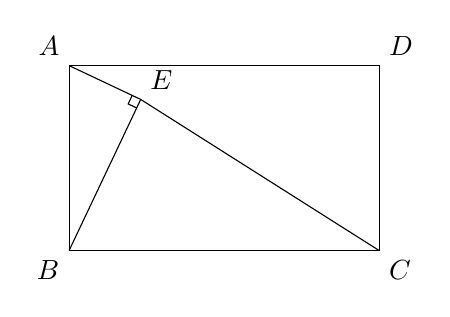
\begin{tikzpicture}
  \coordinate (A) at (0,2.35);
  \coordinate (D) at (3.94,2.35);
  \coordinate (B) at (0,0);
  \coordinate (C) at (3.94,0);
  \coordinate (E) at (0.91,1.92);

  \draw (A) -- (D) -- (C) -- (B) -- cycle;
  \draw (A) -- (E) -- (C);
  \draw (B) -- (E);
  \draw (0.802,1.971) -- (0.751,1.863) -- (0.859,1.812);

  \node[above left] at (A) {$A$};
  \node[above right] at (D) {$D$};
  \node[below left] at (B) {$B$};
  \node[below right] at (C) {$C$};
  \node[above right] at (E) {$E$};
\end{tikzpicture}
\end{document}
